\documentclass[10pt]{exam}
\usepackage{enumerate}
\usepackage{pgfplots}
\usepackage{graphicx, amsmath, amssymb}
\usepgfplotslibrary{polar}
\usepgfplotslibrary{fillbetween}

\title{Integral Applications Test Bank}
\date{}


\begin{document}
\maketitle


\everymath{\displaystyle}

\begin{questions}

\question Consider the region in the first quadrant bounded between $y=x^2$ and $y=2.2x$.  We rotate this region around the $y$ axis to create a solid of revolution.  Which integral below is equal to the volume of that solid using the washer method?


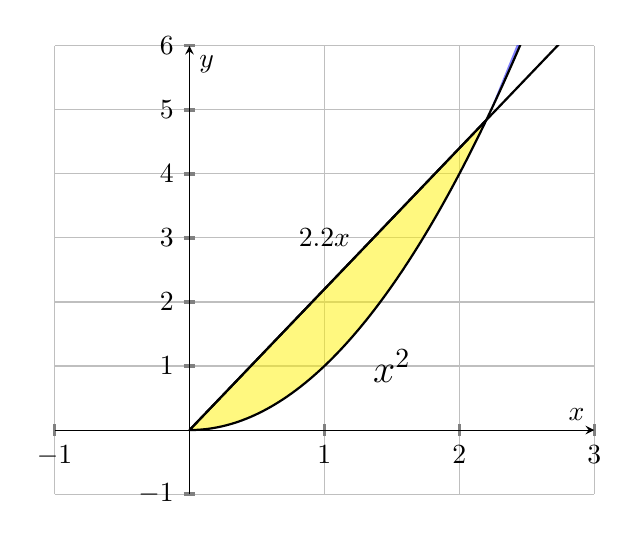
\begin{tikzpicture}
\begin{axis}[
  axis lines=middle,
  grid=major,
  xmin=-1,
  xmax=3,
  ymin=-1,
  ymax=6,
  xlabel=$x$,
  ylabel=$y$,
  xtick={-4,-3,...,4},
  ytick={-2,-1,...,4, 5, 6},
  tick style={very thick},
  legend style={
  at={(rel axis cs:0,1)},
  anchor=north west,draw=none,inner sep=0pt,fill=gray!10}
]

\addplot[thick,samples=100,name path=f][domain=0:3] {x^2} node at (axis cs:1.5,1) {\Large $x^2$};

\addplot[thick,samples=100,domain=0:5] {2.2*x} node at (axis cs:1,3){$2.2x$};


\addplot[thick,samples=100,domain=0:2.2,name path=g] {2.2*x};

\addplot [
        thick,
        color=blue,
        fill=blue, 
        fill opacity=0.5
    ]
    fill between[
        of=f and g,
        split,
        every segment no 0/.style={
            %fill=none,
            yellow,
        },
    ];


\end{axis}
\end{tikzpicture}



\begin{choices} % correct: C

\choice  $\pi \int_0^{2.2} y\left(1-\frac{y}{2.2^2}\right)dy$

\choice  $\pi \int_0^{2.2} y\left(1+\frac{y}{2.2^2}\right)dy$


\choice  $\pi \int_0^{4.84} y\left(1-\frac{y}{2.2^2}\right)dy$ %correct

\choice  $2\pi \int_0^{2.2} (x^2)^2 - (2.2 x)^2  dx$


\choice  $2\pi \int_0^{4.84} (x^2)^2 - (2.2 x)^2  dx$
	
\end{choices}






\question 

Let $f(x) = \sin(x)$ and consider the region bounded between $f$ and the $x$-axis between $x=0$ and $x=\pi$.  What is the volume of the solid given by rotating this region about the $y$-axis? [SHOW ALL YOUR WORK.]



\question  Assume we can apply the Mean Value Theorem to the function f.  Also, assume the average rate of change of $f$ on the interval $[a,b]$ is 14.  Then which of the following statements is true according to the Mean Value Theorem?

\begin{choices}  % correct: C
\choice The derivative of $f$ equals 14;
\choice There is a point $x^*$ in the interval where $f'(x^*) = f(b)-f(a)$;
\choice There is a point in the interval where the derivative equals the average rate of change; %correct
\choice There is a point $x^*$ in the interval where $f'(x^*) = \frac{14}{b-a}$;

\choice Right in the middle, at $x=\frac{a+b}{2}$, the derivative equals 14.
	
\end{choices}


\question Consider a crane from which is suspended a chain.  The chain is 74 meters long and its linear density is 45 kilograms per meter.  How much work is done to the chain in drawing it into the crane?  [SHOW ALL YOUR WORK.  IN YOUR WORK, EXPLAIN HOW WE BUILD A RIEMANN SUM AND HOW WE TURN THAT INTO AN INTEGRAL, AND THEN EVALUATE THE INTEGRAL.]


\includegraphics[width=2in]{images/work_problem}




\question \label{pyr1} Consider a pyramid with a square base.  The base has length 5 meters on each side.  The pyramid is 3 meters tall.  Put coordinates on the pyramid as in the image below.

In the image, we have shaded a cross section of the pyramid at some particular $y$.  Write a formula for $A(y)$, the area of this cross section in terms of $y$ 

\includegraphics[width=2in]{images/pyramid}

\begin{choices}


\choice  $A(y) = \frac{5}{3}(3-y)$
\choice  $A(y) = \frac{25}{9}(3-y)^2$ %correct
\choice $A(y) = \frac{5}{3} y$
\choice $A(y) = \frac{25}{9} y^2$
\choice  $A(y) = \frac{5}{3}(3-y)^2$

\end{choices}



\question Continue Question \ref{pyr1}.  Compute the volume of the pyramid.

\begin{choices}
\choice 14
\choice $\frac{5}{3}$
\choice 25 %correct
\choice $\frac{25}{9}$
\choice $5\pi$
\end{choices}


\question  Consider the function $f(x) = 2x^2$.  Which of the following integrals is equal to the arc length of $f$ between 0 and 1.

\begin{choices}
\choice $\int_0^1 \sqrt{1+(4x)^2} dx$
	\choice $\int_0^1 (1+(4x)^2) dx$
	\choice $\int_0^1 \sqrt{1+(2x^2)^2} dx$
	\choice $\int_0^1 \sqrt{1-(2x^2)^2} dx$
	\choice $2\pi \int_0^1 \sqrt{1+(4x)^2} dx$
\end{choices}



\question T/F Let $f$ be a continuous function.  Assume $f(1)=0$ and $f(2)=0$ and those are the only zeros of this function.  It never equals zero anywhere else. If $f(1.5)=1$, then $f(x)$ is positive on the whole interval $(1,2)$. 

\question Choose the best explanation for this improper Riemann integral:
$$\int_0^\infty \frac{1}{x^2+2}dx$$

\begin{choices}
\choice The integral diverges.
\choice The integral does not exist.
\choice The integral exists and is finite.
\choice The integral oscillates.
\choice The integral is infinite.
	
\end{choices}


\question

Explain how we compute the arc length of a function $f(x)$.  In your explanation, include as much detail as you can.  Draw illustrations and explain in English sentences and write math equations---anything that helps show what you know.






\end{questions}



\end{document}